\chapter{Software development process}
\label{chapter:Analysis tool}

\begin{introduction}
    “I've learned a painful lesson, that for small programs dynamic typing is great. For large programs, you have to have a more disciplined approach. And it helps if the language actually gives you that discipline, rather than telling you, 'Well, you can do whatever you want.'” - Guido van Rossum, Python's creator
\end{introduction}

Falar de Metodologia Agile

\section{Requirements}

This section presents the requirements for the developed software, categorized into functional and non-functional requirements. 
\subsection{Functional Requirements}

Functional requirements specify the functionalities that end-users require as essential components of the system. They describe the system's behavior in terms of inputs, operations to be performed, and expected outcomes. These requirements are directly observable by users in the final product. \cite{Geeks2024} The main functional requirements of the developed software are:

\subsubsection{\textbf{FR1 - Collection of BAM/CRAM Files for Analysis}}

The software must enable the collection of BAM/CRAM sequencing files stored on the company's servers.

\subsubsection{\textbf{FR2 - Calculation of Depth of Coverage/Read Depth and Coverage/Breadth of Coverage}}

The software must facilitate the calculation of Depth of Coverage and Coverage/Breadth of Coverage for the collected BAM/CRAM files. Users should be able to configure analysis parameters, such as selecting regions of interest within the exome. The analysis should be based on a universal BED file containing exon coordinates. The analysis should use bioinformatics tools like SAMtools, which returns a .depth file with results that must be processed by the software to obtain the desired metrics.

\subsubsection{\textbf{FR3 - Graphical User Interface}}

The software must have a graphical user interface that allows users to interact with the system in an intuitive and efficient manner. The interface should be simple and easy to use, enabling users to collect BAM/CRAM files, configure analysis parameters, and view the obtained results. The interface should be developed using Streamlit, a Python web development tool that allows the creation of interactive web applications with minimal code. It should support user interaction through widgets such as buttons, text boxes, sliders, and others. The interface should allow filtering of results and exporting results to a CSV file.

\subsection{Non-Functional Requirements}

Non-functional requirements refer to the quality attributes of the software, such as performance, usability, security, and scalability. These requirements are crucial to ensure that the software operates efficiently, is secure, and can be easily used by various user profiles. \cite{Geeks2024} The main non-functional requirements of the system are described as follows:

\subsubsection{\textbf{NFR1 - Usability}}

The software should be intuitive and user-friendly, enabling even users with no technical background to interact with the system efficiently. The graphical user interface should be simple and clear, with straightforward instructions on how to use the system. It should allow users to collect BAM/CRAM files, configure analysis parameters, and view results quickly and easily. Clear and informative error messages should be provided in case of task execution failures, along with instructions for resolving issues.

\subsubsection{\textbf{NFR2 - Performance}}

The software must be optimized to process large volumes of sequencing data, ensuring that the calculation of Depth of Coverage/Read Depth and Coverage/Breadth of Coverage occurs within a reasonable time frame. The possibility of parallelizing calculations should be explored, utilizing multicore or distributed resources to accelerate data processing.

\subsubsection{\textbf{NFR3 - Scalability}}

The system must be scalable, capable of handling significant increases in data volume or the number of users without compromising performance. This includes the ability to leverage cloud services such as AWS S3. The software should be designed to allow the addition of new modules or functionalities without the need to rewrite the core code, ensuring flexibility for future evolution of the system.

\subsubsection{\textbf{NFR4 - Security and Data Privacy}}

The software must protect sensitive data, especially patient-related data, in compliance with regulations such as General Data Protection Regulation (GDPR). Temporary data used during processing must be properly deleted after analysis, ensuring data privacy and security. System access should be controlled through authentication and authorization, ensuring that only authorized users can interact with the system. A logging system should be implemented to record user activities and monitor system usage.

\subsubsection{\textbf{NFR5 - Portability and Compatibility}}

The software should be implemented on Windows but must ensure access to a Linux environment using WSL. It should guarantee easy integration with tools like Samtools in the WSL environment without requiring advanced configuration by the end user.

\subsubsection{\textbf{NFR6 - Maintainability}}

The software code must be modular and well-documented, facilitating easy maintenance and extension of the system in the future. Best development practices, such as version control (Git), should be applied, ensuring that the code can be managed efficiently over time. Software updates should be simple to implement, and developer documentation should include clear instructions on how to add new functionalities or adjust existing behaviors.

With clear definitions of functional and non-functional requirements, the development of the software was structured efficiently, ensuring it meets both technical expectations and operational needs of the company and end-users. Considering these requirements throughout the development cycle was crucial for the success of the project.



\section{System Design and Architecture}

The developed software is based on a web interface accessible through a browser, using the Streamlit library to build the application. The interface is composed of several interactive widgets that allow the user to configure and execute different types of genomic analysis: Single Gene, Gene Panel, or Exome.

\subsection{User Workflow}

Initially, the user must select the type of analysis they wish to perform. Depending on the selection, the processing flow adapts to optimize both the user experience and the efficiency of the necessary calculations.

\subsubsection{\textbf{Single Gene Analysis}}

The user uploads a BAM or CRAM file, containing the sequencing data. Additionally, they automatically receive a universal BED file corresponding to the selected genome assembly. The user then chooses the gene of interest and may specify the exon(s) to be analyzed. SAMTOOLS is invoked to generate a DEPTH file, which contains information about the read depth at each genomic position. This file is processed by a Python script that calculates two key metrics: depth of coverage and breadth of coverage. The results are displayed to the user through a report in the Streamlit interface or can be exported as a CSV file.

\subsubsection{\textbf{Gene Panel Analysis}}

Similar to the Single Gene analysis, the user uploads a BAM/CRAM file and receives the universal BED file. However, in this case, the user selects the gene panel for the analysis instead of a single gene. The corresponding BED file is processed by SAMTOOLS to generate the DEPTH file, which is then used to calculate the same coverage metrics. The result visualization and export process follow the same steps as in the Single Gene analysis.


\subsubsection{\textbf{Exome Analysis}}

In Exome analysis, the entire exome is used for the analysis, without requiring the selection of a specific region. The user uploads the BAM/CRAM file, and the universal BED file corresponding to the exome is utilized. As in the other modes, SAMTOOLS generates the DEPTH file, which is processed to calculate the coverage metrics. The results are displayed or exported in the same manner.


The modular design of the software allows for seamless integration between various components, namely Streamlit for the interface, SAMTOOLS for processing sequencing data, and Python scripts for calculating coverage metrics. Each of these steps is interconnected to provide the user with quick, accurate, and real-time results. The software's architecture is designed to be easily scalable and adaptable to different types of genomic analysis, supporting both focused and large-scale analyses (such as whole exome).

The Figure \ref{fig:architecture} shows the scheme of the software architecture, highlighting the main components.

\begin{figure}[H]
    \centering
    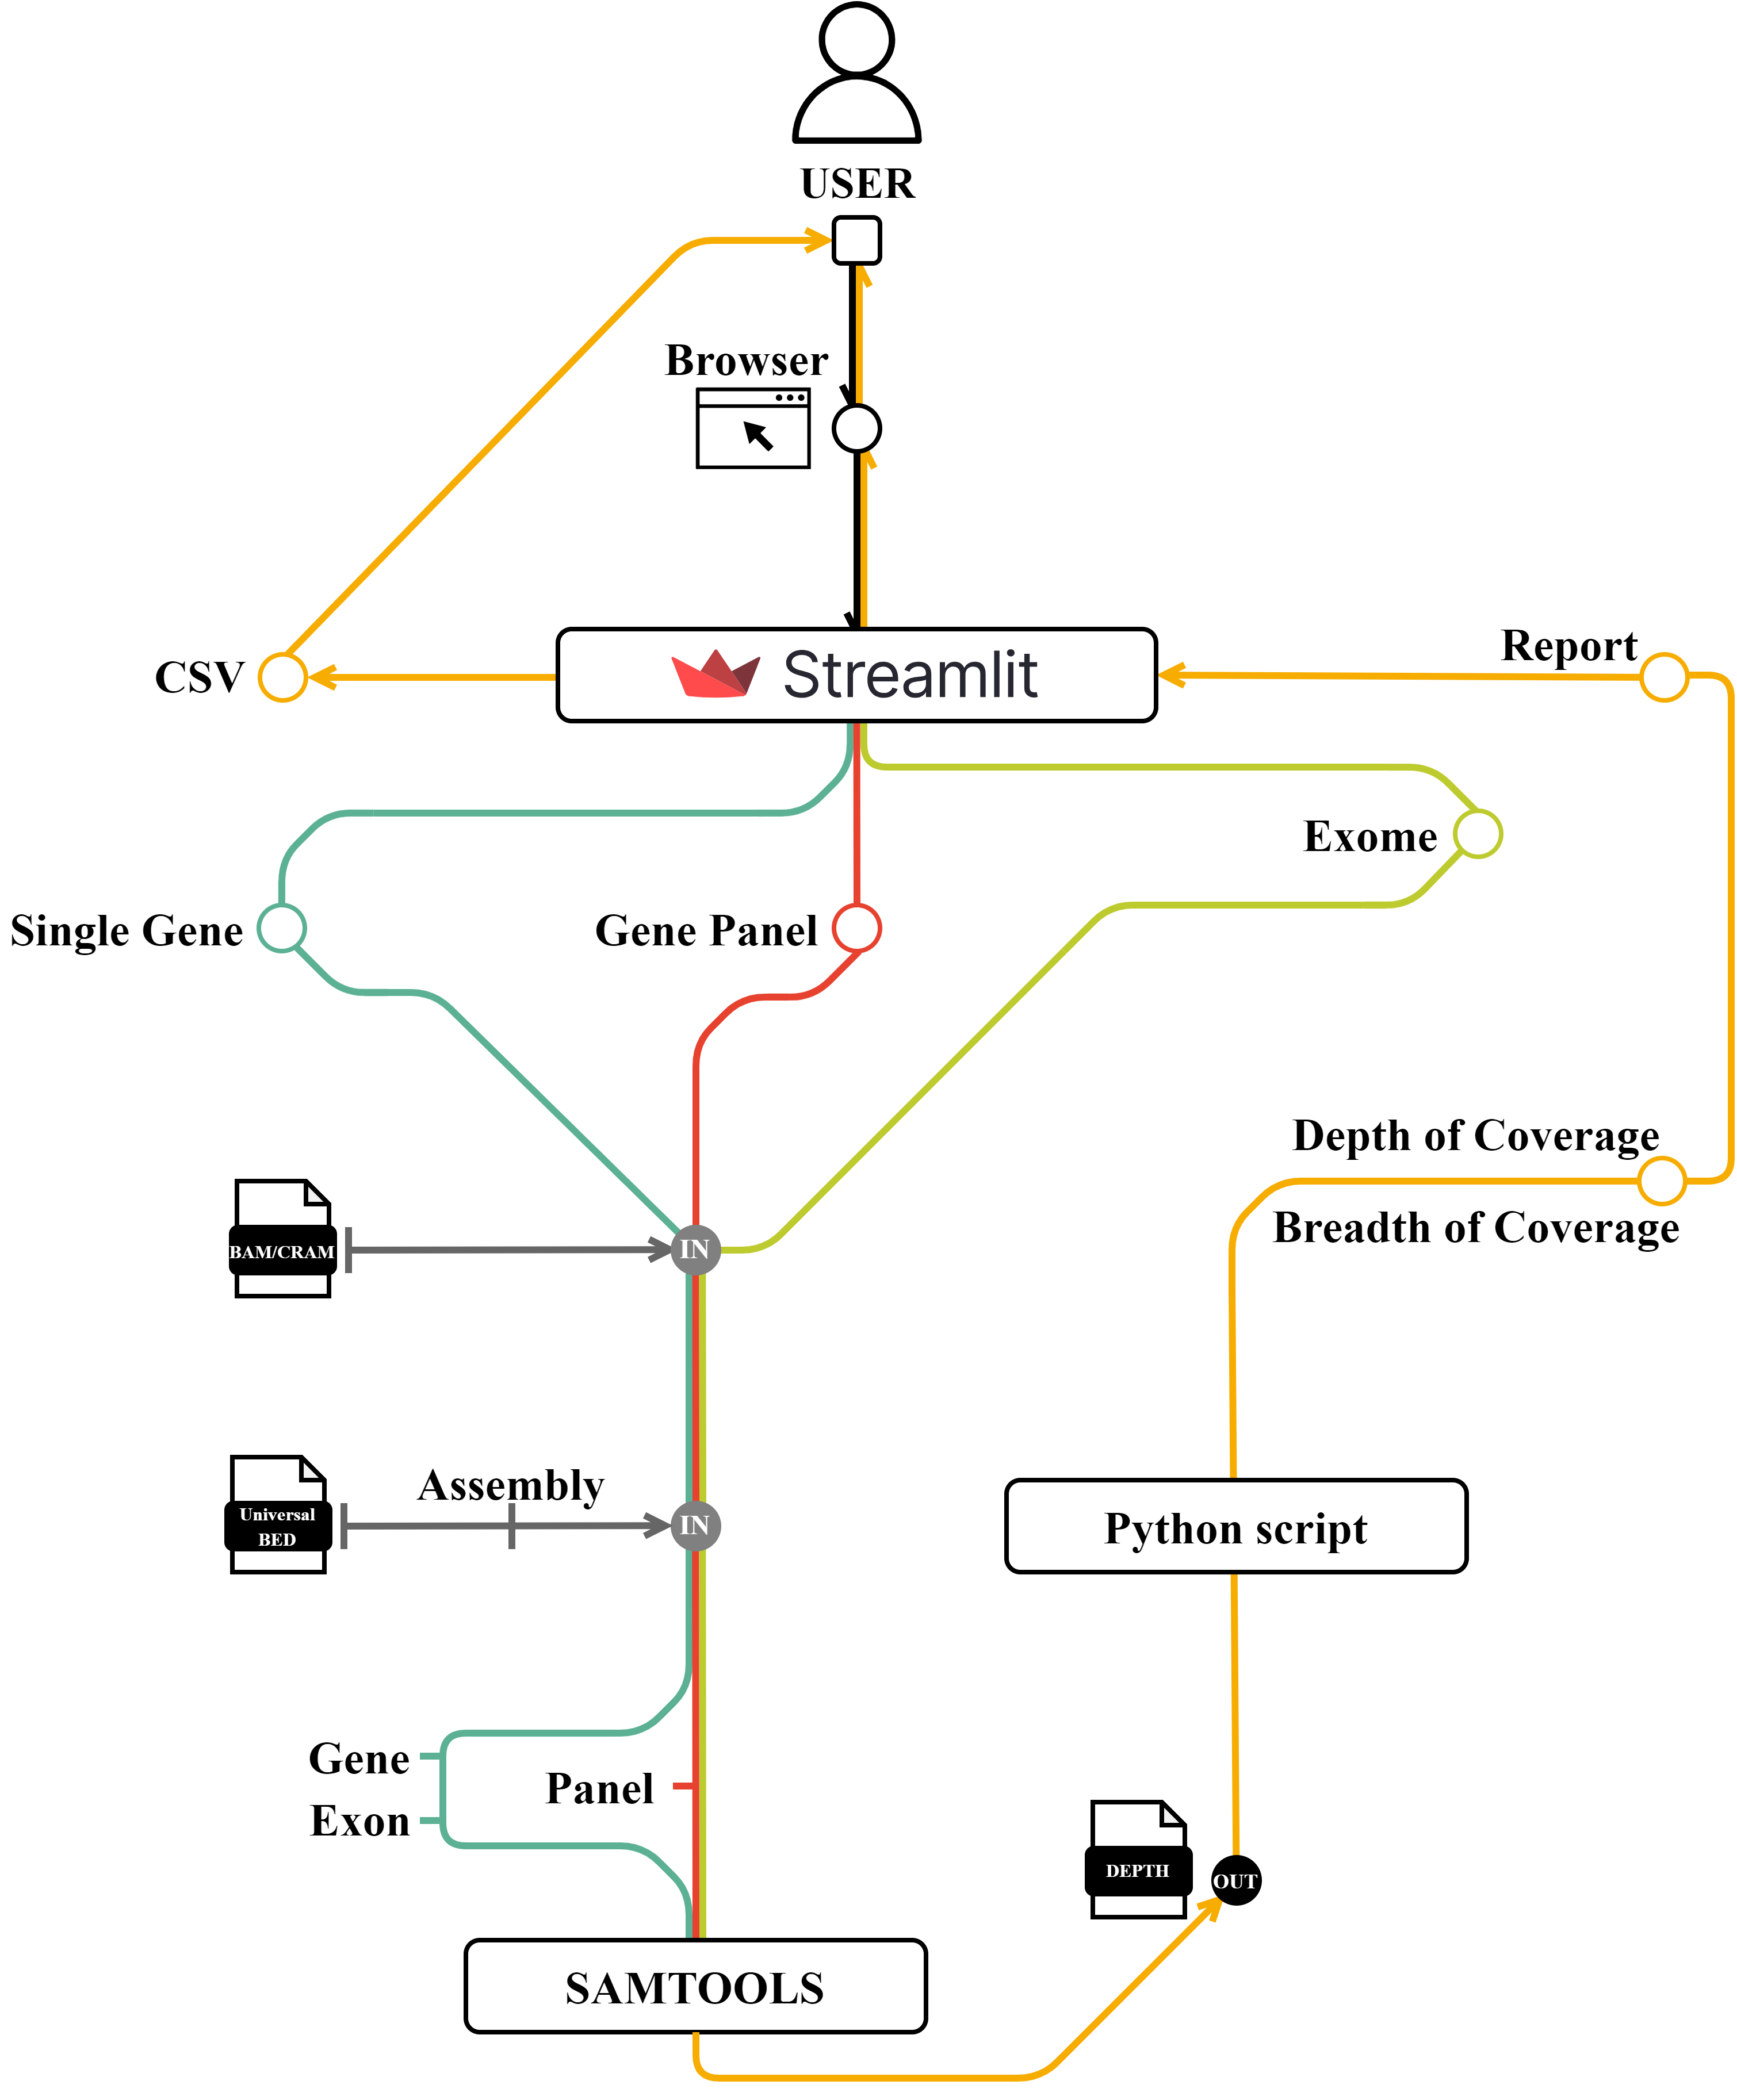
\includegraphics[width=1\textwidth]{figs/architecture.png}
    \caption{Scheme of the software architecture.} 
    \label{fig:architecture}
\end{figure}



\section{Development}

The development of the software followed an iterative and structured approach, with each stage focusing on expanding its functionality while ensuring stability and performance. The process began with the implementation of the Single Gene analysis, which served as the foundation for the project. This initial version was designed to be stable and functional, enabling users to upload BAM or CRAM files and analyze specific genes and exons with precision.

Once the Single Gene functionality was fully operational, the next phase involved adding support for Gene Panel analysis. This required adjusting the existing framework to handle a broader set of genes while maintaining the same level of accuracy and efficiency. A stable and functional version was again achieved, providing users with the ability to select and analyze predefined gene panels.

Finally, the software was further enhanced to include Exome analysis, allowing for the comprehensive examination of the entire exome. This functionality was integrated without compromising the stability or performance of the system, and once again, a stable and functional version was built.

Throughout the development, various components and tools were employed to ensure the software met the required performance standards and provided an intuitive user experience. The careful progression from Single Gene to Gene Panel, and finally to Exome analysis, highlights the modularity and scalability of the software, as well as the emphasis placed on testing and validation at each stage.

The following sections provide an overview of the key tools and technologies used in the development of the whole software, including all the stages of the project.
\subsection{Environment preparation }
\subsubsection{\textbf{Windows Subsystem for Linux (WSL)}}

On Windows, developers have access to both the Windows and Linux environments, thanks to the Windows Subsystem for Linux (WSL). With WSL, it is possible to install different Linux distributions, such as Ubuntu, OpenSUSE, Kali, Debian, Arch Linux, among others. This allows Linux applications, utilities and command-line tools to be used directly in Windows, without the need to modify the operating system, resort to virtual machines or dual boot. \cite{wsl}

In the context of the development of this tool, the need to install WSL was driven mainly due to the scenario in which many essential tools and software for bioinformatics are designed to work in Linux environments. For this reason, we followed the set of steps recommended on the Microsoft website to configure this environment (Build 19041 or higher). \cite{wsl}

\subsubsection{\textbf{Anaconda and Conda}}

After installing WSL, the installation step of Anaconda followed, a platform for data science in Python/R that includes conda, a package and environment manager, making it easier for users to manage a collection of more than 7,500 open source packages. \cite{anaconda1}

In the case of the creation of the metrics analysis tool, this step was fundamental to allow the installation and maintenance of all the packages and dependencies necessary for the operation of the software. By creating a conda environment, it was possible to ensure that all installed tools work independently without conflicts between versions and packages, thus ensuring the reproducibility of the created software. \cite{anaconda2}

Following the documentation provided by Anaconda, the installation and creation of the conda environment was carried out. \cite{anaconda3} 

Additionally, all the dependencies of the attached x-list were installed within the created environment. This installation was carried out by installing package by package, however, an environment.yaml file was made available that allows the bulk installation \cite{anaconda4} of all dependencies on the versions compatible with the software.

\subsubsection{\textbf{Git and GitHub}}

GitHub is a platform that allows users to store, share, and collaborate on code writing with others. \cite{github}

Its operation is based on repositories managed by Git, a version control system that tracks all changes made by one or more users in a project. \cite{github}

When files are uploaded to GitHub, they become part of the created repository. Any change (commit) to any file is automatically tracked. These changes, made locally, are usually synchronized continuously by pushing the committed changes. Similarly, any changes made locally by another user and synchronized on GitHub can be retrieved by making a pull request. \cite{github}

Thus, by using the documentation of Git and GitHub, this practice was implemented, which not only ensures that each version of the created software is recorded—guaranteeing that the work is not lost and allowing for version rollback in case of bugs—but also ensures that all software produced is reproducible and available for deployment by any user. \cite{github}

\subsection{Streamlit}

\subsection{SAMtools}

SAMtools is an essential tool for the manipulation and analysis of DNA sequencing data. First released in 2009, it allows for converting, manipulating, sorting, querying, calculating statistics, calling variants, and analyzing sequencing data in SAM, BAM, and CRAM formats. \cite{samtools}

Among the many functionalities of SAMtools, the most notable are its ability to convert formats, manipulate and index files, visualize and export data, and calculate statistics, such as "depth," which served as the basis for the tool created. \cite{samtools}

In this case, a Python function was developed to generate a .depth file with the desired metrics, using SAMtools depth.

\begin{listing}[h]
\begin{minted}{python}
import subprocess

def depth(bam_path, bed_path, depth_path, gene_selection=None, exon_selection=None): 
    """ 
    Calculate the depth of coverage for specific exons of genes in a BAM file using samtools.
s
    Args: 
        bam_path (str): Path to the BAM file.
        bed_path (str): Path to the Universal BED file containing exon coordinates.
        depth_path (str): Path to save the depth output.
        gene_selection (list or None): List of gene names to include in the depth calculation. 
                                       If None, all genes will be included.
        exon_selection (list or None): List of exon numbers to include in the depth calculation. 
                                       If None, all exons will be included.

    Returns: 
        None
    """ 
    
    gene_filter = ','.join(map(str, gene_selection)) if gene_selection else '' 
    exon_filter = ','.join(map(str, exon_selection)) if exon_selection else ''
    
    # Construct awk command to filter based on gene and exon selection
    awk_command = (f'awk -v gene_filter={gene_filter} -v exon_filter={exon_filter} '
                   f'\'{{split(exon_filter, arr, ","); '
                   f'if (($4 == gene_filter || gene_filter == "") && '
                   f'("" in arr || $5 == arr[1])) {{sub(/^chr/, "", $1); print}}}}\' {bed_path}')
    
    # Construct samtools command to calculate depth
    samtools_command = f'samtools depth -b - {bam_path} > {depth_path}'
    
    # Run the commands using subprocess
    try:
        subprocess.run(f'{awk_command} | {samtools_command}', shell=True, check=True)
    except subprocess.CalledProcessError as e:
        print(f"Error occurred: {e}")
\end{minted}
\caption{Python function to calculate depth of coverage using samtools and awk.}
\label{lbl:snippet-test}
\end{listing}

\subsection{Python script for metrics calculation}

\section{Test and validation}

\section{Feedback and Iteration???}

\section{Optimization}

\section{Deployment}


\section{Impact on the company}